% This file was created with tikzplotlib v0.10.1.
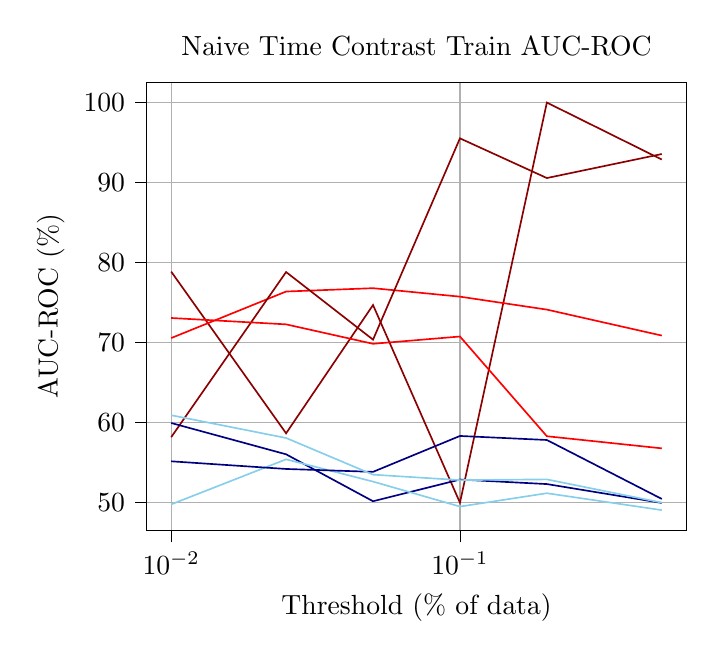
\begin{tikzpicture}

\definecolor{darkgray176}{RGB}{176,176,176}
\definecolor{darkred}{RGB}{139,0,0}
\definecolor{navy}{RGB}{0,0,128}
\definecolor{skyblue}{RGB}{135,206,235}

\begin{axis}[
log basis x={10},
tick align=outside,
tick pos=left,
title={Naive Time Contrast Train AUC-ROC},
x grid style={darkgray176},
xlabel={Threshold (\% of data)},
xmajorgrids,
xmin=0.00822340159426889, xmax=0.608020895329329,
xmode=log,
xtick style={color=black},
xtick={0.0001,0.001,0.01,0.1,1,10},
xticklabels={
  $\mathdefault{10^{-4}}$,
  $\mathdefault{10^{-3}}$,
  $\mathdefault{10^{-2}}$,
  $\mathdefault{10^{-1}}$,
  $\mathdefault{10^{0}}$,
  $\mathdefault{10^{1}}$
},
y grid style={darkgray176},
ylabel={AUC-ROC (\%)},
ymajorgrids,
ymin=46.5217280692688, ymax=102.539951778429,
ytick style={color=black}
]
\addplot [semithick, darkred]
table {%
0.01 78.869874185823
0.025 58.6651904160833
0.05 74.6977327837147
0.1 50
0.2 99.9936688825578
0.5 92.8718779357544
};
\addplot [semithick, red]
table {%
0.01 70.5669748286852
0.025 76.3819532096678
0.05 76.7994796604708
0.1 75.7423841190858
0.2 74.1232448786277
0.5 70.8779172652567
};
\addplot [semithick, darkred]
table {%
0.01 58.1806270204352
0.025 78.8166894866511
0.05 70.3682121267776
0.1 95.5225020481942
0.2 90.5619701564469
0.5 93.5632873792363
};
\addplot [semithick, red]
table {%
0.01 73.0748156595876
0.025 72.2791446805349
0.05 69.8511153531738
0.1 70.7612490588157
0.2 58.3006943985334
0.5 56.7862553026482
};
\addplot [semithick, navy]
table {%
0.01 59.9548411440192
0.025 56.0425727092522
0.05 50.1765596400447
0.1 52.8874280104395
0.2 52.3226336047648
0.5 49.9657039301467
};
\addplot [semithick, skyblue]
table {%
0.01 49.7852536425519
0.025 55.4150816823367
0.05 52.6326103595733
0.1 49.5100151872444
0.2 51.1806831389973
0.5 49.0680109651397
};
\addplot [semithick, navy]
table {%
0.01 55.1684312691669
0.025 54.2104702705058
0.05 53.8488586977808
0.1 58.3342824161328
0.2 57.8304726800747
0.5 50.464719844418
};
\addplot [semithick, skyblue]
table {%
0.01 60.9253483317186
0.025 58.0805036592072
0.05 53.4988279511672
0.1 52.8176774059731
0.2 52.9088241358443
0.5 50
};
\end{axis}

\end{tikzpicture}
